\documentclass[11pt,a4paper]{article}

% ----------------------------------------------------------------------
% Page Geometry and Layout
% ----------------------------------------------------------------------
\usepackage[margin=2.2cm, top=2.3cm, bottom=2.3cm]{geometry}

% ----------------------------------------------------------------------
% Typography and Fonts
% ----------------------------------------------------------------------
\usepackage{mathptmx}             % Times Roman text and matching math font
\usepackage[scaled=0.92]{helvet}  % Clean Helvetica for sans-serif
\usepackage{courier}              % Courier for monospace
\usepackage[T1]{fontenc}
\usepackage[utf8]{inputenc}
\usepackage{microtype}
\usepackage{parskip}
\setlength{\parindent}{0pt}
\setlength{\parskip}{5.5pt}

% ----------------------------------------------------------------------
% Mathematical Packages
% ----------------------------------------------------------------------
\usepackage{amsmath, amssymb}
\usepackage{bm}

% ----------------------------------------------------------------------
% Tables and Lists
% ----------------------------------------------------------------------
\usepackage{booktabs}
\usepackage{tabularx}
\usepackage{array}
\usepackage{colortbl}
\usepackage{float}
\usepackage{enumitem}
\setlist{nosep, leftmargin=1.5em}

% ----------------------------------------------------------------------
% Caption Formatting
% ----------------------------------------------------------------------
\usepackage{caption}
\captionsetup{
    labelfont={bf,sf,color=primary},
    textfont={small},
    labelsep=colon,
    skip=7pt
}

% ----------------------------------------------------------------------
% Colors and Visual Elements
% ----------------------------------------------------------------------
\usepackage{xcolor}
\definecolor{primary}{RGB}{15, 44, 89}      % Deep Navy Blue
\definecolor{secondary}{RGB}{31, 110, 140}  % Slate Blue
\definecolor{accent}{RGB}{43, 91, 169}     % Royal Accent
\definecolor{lightbg}{RGB}{246, 248, 250}   % Soft Neutral Light Gray
\definecolor{darkslate}{RGB}{33, 37, 41}   % Charcoal Text
\definecolor{alertred}{RGB}{192, 41, 43}    % Structured Warning Red
\definecolor{successgreen}{RGB}{39, 174, 96}% Success Green
\definecolor{codebg}{RGB}{240, 243, 246}    % Code Box Background
\definecolor{frameborder}{RGB}{209, 217, 224}

\usepackage{graphicx}
\usepackage{tikz}
\usetikzlibrary{shapes.geometric, arrows.meta, positioning, calc, fit, backgrounds, patterns}

% ----------------------------------------------------------------------
% Boxes and Callouts (tcolorbox)
% ----------------------------------------------------------------------
\usepackage{tcolorbox}
\tcbuselibrary{skins, breakable}

\newtcolorbox{terminalbox}[1][]{%
    colback=codebg,
    colframe=primary,
    coltitle=white,
    fonttitle=\bfseries\small\sffamily,
    title={#1},
    sharp corners,
    boxrule=1pt,
    left=8pt, right=8pt, top=6pt, bottom=6pt,
    fontupper=\ttfamily\footnotesize,
    breakable
}

\newtcolorbox{summarybox}[1][]{%
    colback=lightbg,
    colframe=secondary,
    coltitle=white,
    fonttitle=\bfseries\small\sffamily,
    title={#1},
    sharp corners,
    boxrule=1pt,
    left=9pt, right=9pt, top=6pt, bottom=6pt,
    fontupper=\small,
    breakable
}

% ----------------------------------------------------------------------
% Section Heading Styling (titlesec)
% ----------------------------------------------------------------------
\usepackage{titlesec}
\titleformat{\section}
  {\color{primary}\normalfont\Large\bfseries\sffamily}
  {\thesection}{1em}{}[\color{primary}\titlerule]
\titlespacing*{\section}{0pt}{11pt plus 2pt minus 2pt}{5pt plus 1pt minus 1pt}

\titleformat{\subsection}
  {\color{secondary}\normalfont\large\bfseries\sffamily}
  {\thesubsection}{0.8em}{}
\titlespacing*{\subsection}{0pt}{8pt plus 2pt minus 1pt}{3pt plus 1pt minus 1pt}

\titleformat{\subsubsection}
  {\color{darkslate}\normalfont\normalsize\bfseries\sffamily}
  {\thesubsubsection}{0.6em}{}
\titlespacing*{\subsubsection}{0pt}{6pt plus 1pt minus 1pt}{2.5pt plus 1pt minus 1pt}

% ----------------------------------------------------------------------
% Headers and Footers (fancyhdr)
% ----------------------------------------------------------------------
\usepackage{fancyhdr}
\pagestyle{fancy}
\setlength{\headheight}{14.5pt}
\fancyhf{}
\fancyhead[L]{\small\textbf{\color{primary}PortScan-OS} \ $\cdot$ \ {\color{secondary}Project Design Report}}
\fancyhead[R]{\small\color{darkslate!80}CSE 406 $\cdot$ 2105032 $\cdot$ 2105033}
\fancyfoot[L]{\small\color{darkslate!75}Port Scanning with OS Detection and Exploitation}
\fancyfoot[R]{\small\bfseries\color{primary}Page \thepage}
\renewcommand{\headrulewidth}{0.75pt}
\renewcommand{\headrule}{%
  \vskip 2.5pt%
  {\color{secondary!60}\hrule height \headrulewidth width \headwidth}%
  \vskip -\headrulewidth%
}
\renewcommand{\footrulewidth}{0.4pt}
\renewcommand{\footrule}{{\color{frameborder}\hrule height \footrulewidth width \headwidth \vskip-\footrulewidth}}

% ----------------------------------------------------------------------
% Hyperlinks
% ----------------------------------------------------------------------
\usepackage[
    colorlinks=true,
    linkcolor=primary,
    citecolor=secondary,
    urlcolor=accent,
    bookmarksnumbered=true
]{hyperref}

% ----------------------------------------------------------------------
% Document Body
% ----------------------------------------------------------------------
\begin{document}

% ----------------------------------------------------------------------
% Cover Page (Page 1)
% ----------------------------------------------------------------------
\thispagestyle{empty}

% Top-Right Header Block
\begin{flushright}
    {\color{darkslate!75}\large\scshape CYBER SECURITY PROJECT DESIGN REPORT}\\[4pt]
    {\color{darkslate!85}\normalsize\bfseries CSE406 -- Cyber Security Sessional}
\end{flushright}

\vspace*{2.0cm}

% Hero Title with Left Vertical Accent Bar
\noindent
{\color{secondary}\vrule width 5.5pt}%
\hspace*{18pt}%
\begin{minipage}{\dimexpr\textwidth-26pt\relax}
    {\fontsize{34pt}{40pt}\selectfont\bfseries\color{primary} PortScan-OS}\\[10pt]
    {\LARGE\bfseries\color{secondary} Port Scanning with OS Information and Version Detection}\\[10pt]
    {\large\itshape\color{darkslate} A Custom Attack Toolkit and Defensive Countermeasure Architecture from Scratch}
\end{minipage}

\vspace*{2.0cm}

% Metadata Block (Left-Aligned, Bold Blue Labels)
\noindent
{\large\setlength{\tabcolsep}{14pt}\renewcommand{\arraystretch}{1.3}
\begin{tabular}{@{}ll@{}}
    \textbf{\color{secondary} Assigned Topic:}        & 8 \\
    \textbf{\color{secondary} Topic Title:}        & Port Scanning with OS information / version \\
    \textbf{\color{secondary} Subsection:}   & A2 \\
    \textbf{\color{secondary} Supervisor:}   & \textbf{Anwarul Bashir Shuaib} \\
    \textbf{\color{secondary} Submitted By:} & \textbf{Nawriz Ahmed Turjo (2105032)} \\
                                             & \textbf{Abhishek Roy (2105033)} \\
\end{tabular}}

\vfill

% Bottom Summary Box
\noindent
\begin{tcolorbox}[
    colback=lightbg,
    colframe=secondary!55,
    arc=3pt,
    boxrule=1.1pt,
    left=20pt, right=20pt, top=14pt, bottom=14pt
]
    \centering
    {\bfseries\Large\color{secondary} Core Attack Pipeline \& Defensive Countermeasures}\\[12pt]
    \normalsize
    \renewcommand{\arraystretch}{1.4}
    \begin{tabular*}{\linewidth}{@{\extracolsep{\fill}}lr@{}}
        \textbf{Raw Layer-2 TCP SYN Port Scanner} & \textbf{Heuristic TCP/IP OS Fingerprinting} \\[4pt]
        Stream Banner Grabbing (FTP \& HTTP) & Sliding-Window Dynamic Firewall Defense \\
    \end{tabular*}
\end{tcolorbox}

\vspace*{1.0cm}

\clearpage

% ----------------------------------------------------------------------
% 1. Overview of the Project Idea
% ----------------------------------------------------------------------
\section{Overview of the Project Idea}

\subsection{Problem Statement and Threat Model}
Network reconnaissance determines which communication channels and service ports are reachable across a network perimeter, what software daemon versions run on those ports, and what operating system kernel manages the host. While off-the-shelf tools like Nmap automate this process, building a custom reconnaissance engine demonstrates how raw packets are serialized and parsed on Windows. Operating within an adjacent local subnet, this toolkit manually constructs Ethernet, IPv4, and TCP frames to identify reachable ports, fingerprint the host operating system, and validate exposed services within defined safety limits.

\subsection{Project Scope and Five-Phase Attack Chain}
The project organizes its workflow into five attack phases alongside a concurrent defensive module:

\begin{table}[H]
\centering
\footnotesize
\renewcommand{\arraystretch}{1.0}
\caption{Five-Phase Reconnaissance and Attack Architecture}
\label{tab:phases}
\begin{tabularx}{\textwidth}{>{\centering\arraybackslash\bfseries}p{1.2cm} >{\raggedright\arraybackslash\bfseries}p{2.7cm} >{\raggedright\arraybackslash}p{3.2cm} >{\raggedright\arraybackslash}X}
\toprule
\textbf{Phase} & \textbf{Designation} & \textbf{Operational Focus} & \textbf{Engineering Mechanism} \\
\midrule
1 & TCP SYN Port Scan & Detect Open, Closed, and Filtered ports & Raw Layer-2 frame construction via Npcap; half-open scan without completing the 3-way handshake. \\
\rowcolor{lightbg}
2 & Banner Grabbing & Service and version identification & Standard stream sockets querying listening daemons (passive capture for FTP, active HTTP probes). \\
3 & OS Fingerprinting & Identify target host operating system & Dual-candidate heuristic scoring of SYN/ACK and RST headers: TTL, window size, RFC 6864 IP ID, and option ordering. \\
\rowcolor{lightbg}
4 & Vulnerability Match & Map findings to attack surfaces & Automated mapping between extracted daemon versions and known proof-of-concept exploit vectors. \\
5 & Exploit Execution & Demonstrate concrete security compromise & Automated dispatch of anonymous FTP authentication and HTTP directory path traversal payloads. \\
\midrule
\textbf{Defense} & \textbf{Scan Detection \& Block} & Passive detection and dynamic mitigation & Sliding-window inspection tracking SYN packet rates and port diversity with dynamic Windows Firewall mitigation. \\
\bottomrule
\end{tabularx}
\end{table}
\vspace{-4pt}

\subsection{Core Design Principles}
The attack and defense modules adhere to four core architectural constraints:
\begin{itemize}[nosep, itemsep=1pt, leftmargin=1.5em]
    \item \textbf{From-Scratch Packet Assembly:} Serializes raw Ethernet II, IPv4, and TCP headers byte by byte in binary format without high-level packet construction libraries.
    \item \textbf{RFC 1071 Checksum Computation:} Computes 16-bit one's complement checksums over IPv4 headers and TCP pseudo-headers using a custom mathematical routine.
    \item \textbf{Npcap Low-Level Driver Interface:} Uses Npcap via Python \texttt{ctypes} strictly for link-layer frame transmission and promiscuous capture on Windows.
    \item \textbf{Integrated Host Defense:} Pairs offensive reconnaissance with a concurrent monitor that detects active scanning and dynamically injects firewall quarantine rules.
\end{itemize}
\vspace{-2pt}

\subsection{Safety Architecture and Operational Safeguards}
To maintain ethical standards and prevent disruption in laboratory networks, the toolkit enforces five non-bypassable safeguards:
\begin{enumerate}[nosep, itemsep=1pt, leftmargin=1.5em]
    \item \textbf{RFC 1918 Scope Validation:} Targets must belong to RFC~1918 private subnets (\texttt{10.0.0.0/8}, \texttt{172.16.0.0/12}, \texttt{192.168.0.0/16}); external destinations are rejected immediately.
    \item \textbf{Bounded Probe Horizon:} Caps probe lists at 50 ports per run ($\text{MAX\_PROBES} = 50$), prohibiting full 65,535-port scans and subnet sweeps.
    \item \textbf{Mandatory Rate Limiting:} Enforces an inter-packet delay $\ge 0.2$\,s (default: 0.5\,s) to avoid buffer saturation or switch broadcast storms.
    \item \textbf{Source Port and Sequence Randomization:} Rotates ephemeral source ports with randomized initial sequence numbers to prevent state collision.
    \item \textbf{Non-Destructive Read-Only Exploits:} Restricts exploit modules to read-only checks (FTP \texttt{PWD}/\texttt{LIST} and HTTP static file traversal).
\end{enumerate}

\clearpage

% ----------------------------------------------------------------------
% 2. Network Topology and Components
% ----------------------------------------------------------------------
\section{Network Topology and System Components}

\subsection{Laboratory Network Architecture}
The experimental testbed operates within an isolated private local subnet (\texttt{192.168.0.0/24}) on a dedicated physical switch. All nodes share the same Layer-2 broadcast domain because the custom scanner crafts raw Ethernet frames and issues direct Address Resolution Protocol (ARP) queries to resolve target hardware addresses.

To evaluate OS fingerprinting across diverse TCP/IP implementations, the testbed incorporates four physical target platforms representing major operating system families, as detailed in Table~\ref{tab:testbed_devices}.

\begin{table}[H]
\centering
\small
\renewcommand{\arraystretch}{1.18}
\caption{Heterogeneous Target Device Specifications in the Laboratory Testbed}
\label{tab:testbed_devices}
\begin{tabularx}{\textwidth}{>{\raggedright\arraybackslash\bfseries}p{2.6cm} >{\raggedright\arraybackslash}p{3.1cm} >{\centering\arraybackslash}p{2.9cm} >{\raggedright\arraybackslash}X}
\toprule
\textbf{Device Role} & \textbf{Operating System Stack} & \textbf{Assigned IPv4} & \textbf{Active Services \& Verification Role} \\
\midrule
Attacker Station & Windows 11 Pro (x86\_64) & \texttt{192.168.0.105} & Toolkit orchestrator, raw Npcap packet injection, and capture monitoring. \\
\rowcolor{lightbg}
Primary Victim & Windows 11 Pro (Build 22631) & \texttt{192.168.0.116} & Vulnerable FTP (:21), HTTP (:80), and dynamic Windows Firewall quarantine agent. \\
Secondary Victim & Apple iPadOS 17 (Darwin BSD) & \texttt{192.168.0.152} & VLC HTTP Sharing (:80); evaluates Darwin option sequence ($\text{WS} < \text{TS}$) and initial TTL 64. \\
\rowcolor{lightbg}
Mobile Target & Android 14 (Linux Kernel 5.x) & \texttt{192.168.0.169} & WiFi FTP Server (:2221); evaluates Linux option layout, RFC 6864 $\text{IP ID} = 0$, and closed RST. \\
Network Appliance & Embedded Linux (Gateway Router) & \texttt{192.168.0.1} & DNS (:53) and HTTP Gateway (:80); evaluates embedded appliance TTL and window defaults. \\
\bottomrule
\end{tabularx}
\end{table}

\begin{figure}[H]
\centering
\resizebox{0.98\linewidth}{!}{%
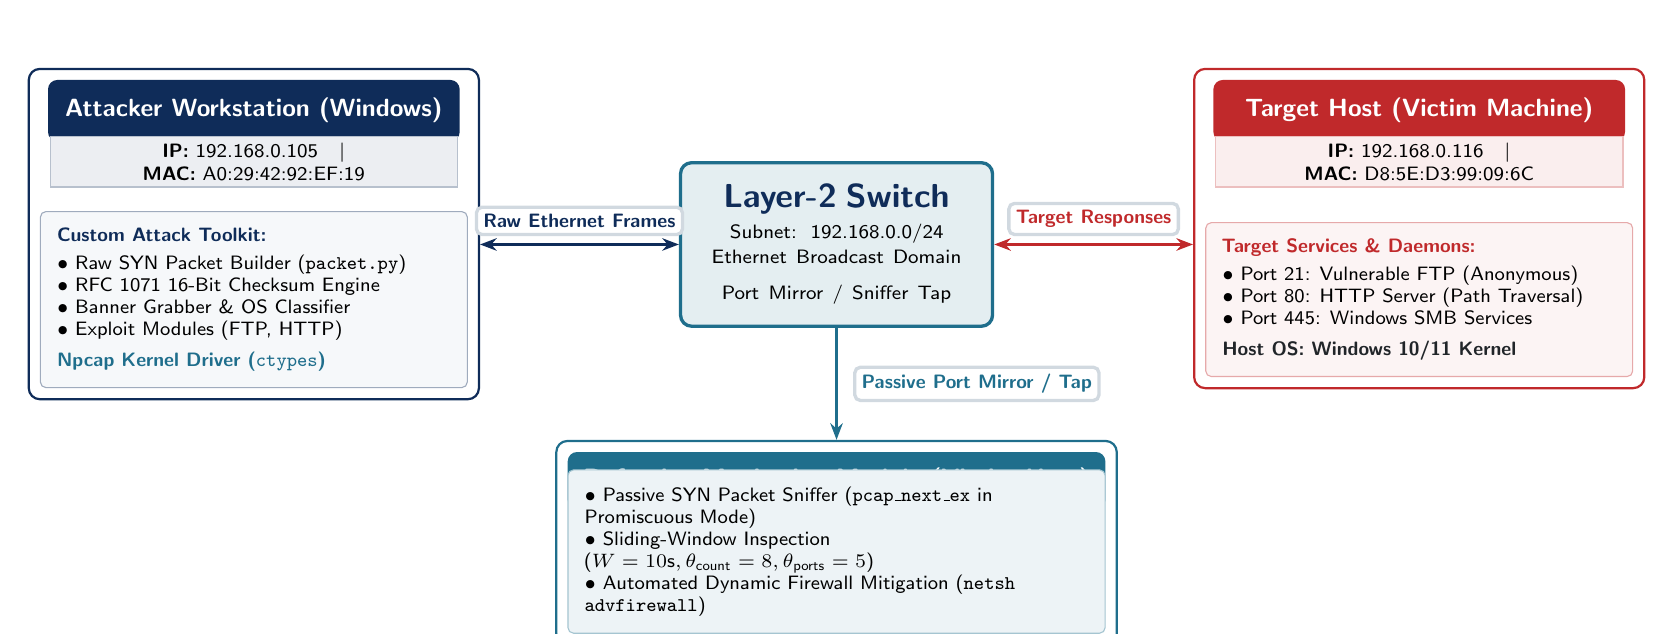
\begin{tikzpicture}[
    font=\sffamily,
    line/.style={draw=darkslate, very thick}
]
    % ------------------------------------------------------------------
    % Left Card: Attacker Machine
    % ------------------------------------------------------------------
    \node[draw=primary, thick, fill=primary, text=white, rounded corners=3pt, minimum width=5.2cm, minimum height=0.75cm, font=\sffamily\bfseries\small] (atk_hdr) at (0, 2.1) {Attacker Workstation (Windows)};
    \node[draw=primary!30, fill=primary!8, font=\sffamily\scriptsize, text width=5.0cm, align=center, inner sep=2.5pt] (atk_sub) at (0, 1.45) {\textbf{IP:} 192.168.0.105 \ \ $\vert$ \ \ \textbf{MAC:} A0:29:42:92:EF:19};
    \node[draw=primary!40, fill=lightbg, font=\sffamily\scriptsize, text width=5.0cm, align=flush left, inner sep=6pt, rounded corners=2pt] (atk_body) at (0, -0.3) {
        \textbf{\color{primary}Custom Attack Toolkit:}\\[2pt]
        $\bullet$ Raw SYN Packet Builder (\texttt{packet.py})\\
        $\bullet$ RFC 1071 16-Bit Checksum Engine\\
        $\bullet$ Banner Grabber \& OS Classifier\\
        $\bullet$ Exploit Modules (FTP, HTTP)\\[3pt]
        \textbf{\color{secondary}Npcap Kernel Driver (\texttt{ctypes})}
    };
    \node[draw=primary, thick, rounded corners=4pt, fit=(atk_hdr) (atk_sub) (atk_body), inner sep=4pt] (atk_card) {};

    % ------------------------------------------------------------------
    % Center: Layer-2 Switch
    % ------------------------------------------------------------------
    \node[draw=secondary, very thick, fill=secondary!12, rounded corners=4pt, text width=3.4cm, align=center, inner sep=8pt] (switch) at (7.4, 0.4) {
        \textbf{\color{primary}\large Layer-2 Switch}\\[3pt]
        {\scriptsize Subnet: 192.168.0.0/24\\[1pt]
        Ethernet Broadcast Domain\\[1pt]
        Port Mirror / Sniffer Tap}
    };

    % ------------------------------------------------------------------
    % Right Card: Victim Machine
    % ------------------------------------------------------------------
    \node[draw=alertred, thick, fill=alertred, text=white, rounded corners=3pt, minimum width=5.2cm, minimum height=0.75cm, font=\sffamily\bfseries\small] (vic_hdr) at (14.8, 2.1) {Target Host (Victim Machine)};
    \node[draw=alertred!30, fill=alertred!8, font=\sffamily\scriptsize, text width=5.0cm, align=center, inner sep=2.5pt] (vic_sub) at (14.8, 1.45) {\textbf{IP:} 192.168.0.116 \ \ $\vert$ \ \ \textbf{MAC:} D8:5E:D3:99:09:6C};
    \node[draw=alertred!40, fill=alertred!5, font=\sffamily\scriptsize, text width=5.0cm, align=flush left, inner sep=6pt, rounded corners=2pt] (vic_body) at (14.8, -0.3) {
        \textbf{\color{alertred}Target Services \& Daemons:}\\[2pt]
        $\bullet$ Port 21: Vulnerable FTP (Anonymous)\\
        $\bullet$ Port 80: HTTP Server (Path Traversal)\\
        $\bullet$ Port 445: Windows SMB Services\\[3pt]
        \textbf{\color{darkslate}Host OS: Windows 10/11 Kernel}
    };
    \node[draw=alertred, thick, rounded corners=4pt, fit=(vic_hdr) (vic_sub) (vic_body), inner sep=4pt] (vic_card) {};

    % ------------------------------------------------------------------
    % Bottom Card: Defensive Monitoring Module
    % ------------------------------------------------------------------
    \node[draw=secondary, thick, fill=secondary, text=white, rounded corners=3pt, minimum width=6.8cm, minimum height=0.7cm, font=\sffamily\bfseries\small] (def_hdr) at (7.4, -2.6) {Defensive Monitoring Module (Victim Host)};
    \node[draw=secondary!40, fill=secondary!8, font=\sffamily\scriptsize, text width=6.4cm, align=flush left, inner sep=6pt, rounded corners=2pt] (def_body) at (7.4, -3.5) {
        $\bullet$ Passive SYN Packet Sniffer (\texttt{pcap\_next\_ex} in Promiscuous Mode)\\
        $\bullet$ Sliding-Window Inspection ($W = 10\text{s}, \theta_{\text{count}} = 8, \theta_{\text{ports}} = 5$)\\
        $\bullet$ Automated Dynamic Firewall Mitigation (\texttt{netsh advfirewall})
    };
    \node[draw=secondary, thick, rounded corners=4pt, fit=(def_hdr) (def_body), inner sep=4pt] (def_card) {};

    % ------------------------------------------------------------------
    % Interconnecting Lines with Dedicated Pill Badges
    % ------------------------------------------------------------------
    \draw[{Stealth[length=6pt]}-{Stealth[length=6pt]}, very thick, color=primary] 
        (atk_card.east |- switch.center) -- (switch.west) 
        node[midway, above=3pt, font=\sffamily\scriptsize\bfseries, fill=white, inner sep=2.5pt, rounded corners=2pt, draw=frameborder] {Raw Ethernet Frames};

    \draw[{Stealth[length=6pt]}-{Stealth[length=6pt]}, very thick, color=alertred] 
        (switch.east) -- (vic_card.west |- switch.center) 
        node[midway, above=3pt, font=\sffamily\scriptsize\bfseries, fill=white, inner sep=2.5pt, rounded corners=2pt, draw=frameborder] {Target Responses};

    \draw[-{Stealth[length=6pt]}, very thick, color=secondary] 
        (switch.south) -- (def_card.north) 
        node[midway, right=6pt, font=\sffamily\scriptsize\bfseries, fill=white, inner sep=2.5pt, rounded corners=2pt, draw=frameborder] {Passive Port Mirror / Tap};

\end{tikzpicture}%
}
\caption{Laboratory Network Topology, Host Roles, and Traffic Monitoring Architecture}
\label{fig:topology}
\end{figure}

\vspace{6pt}
\subsection{Component Specifications}
\begin{table}[H]
\centering
\small
\renewcommand{\arraystretch}{1.24}
\caption{System Component Inventory and Operational Responsibilities}
\label{tab:components}
\begin{tabularx}{\textwidth}{>{\raggedright\arraybackslash\bfseries}p{2.8cm} >{\raggedright\arraybackslash}p{2.2cm} >{\raggedright\arraybackslash}p{4.2cm} >{\raggedright\arraybackslash}X}
\toprule
\textbf{Component} & \textbf{Host Machine} & \textbf{Software Basis} & \textbf{Role in Evaluation} \\
\midrule
SYN Scanner & Attacker & Python / \texttt{packet.py} & Builds raw Ethernet/IPv4/TCP frames, dispatches SYN packets, and logs responses. \\
\rowcolor{lightbg}
Banner Grabber & Attacker & Python / \texttt{banner.py} & Performs stream handshakes to capture service banners from open ports. \\
OS Classifier & Attacker & Python / \texttt{fingerprint.py} & Parses SYN/ACK attributes to calculate operating system probability scores. \\
\rowcolor{lightbg}
Exploit Suite & Attacker & Python / \texttt{exploits/} & Executes targeted exploit modules against confirmed vulnerable ports. \\
Npcap Driver & Attacker/Victim & Npcap Native DLLs & Provides low-level kernel packet capture and raw transmission interfaces. \\
\rowcolor{lightbg}
Vulnerable FTP & Victim & Python / \texttt{ftp\_server.py} & Simulates standard RFC 959 FTP with anonymous read authorization. \\
Vulnerable HTTP & Victim & Python / \texttt{http\_server.py} & Web server with intentional path traversal vulnerability (CVE-2021-41773 analogue). \\
\rowcolor{lightbg}
Defense Monitor & Victim & Python / \texttt{detector.py} & Passive traffic sniffer calculating sliding-window SYN probe arrival rates. \\
Firewall Agent & Victim & Windows \texttt{netsh} & Injects dynamic inbound blocking rules when scanning thresholds are breached. \\
\bottomrule
\end{tabularx}
\end{table}

\subsection{Link-Layer Hardware Address Resolution Architecture}
Constructing raw Layer-2 Ethernet II frames requires both the source MAC address of the local network interface and the destination MAC address of the target host. Because standard Python socket libraries on Windows do not expose link-layer address tables directly, the system queries the Windows IP Helper library (\texttt{iphlpapi.dll}) through \texttt{ctypes}:

\begin{enumerate}[nosep, leftmargin=1.5em]
    \item \textbf{Local Interface and Source MAC Discovery:} The scanner identifies the active network interface by opening an ephemeral UDP probe to the target subnet and reading the bound local IP address. It then calls \texttt{GetAdaptersInfo()} to extract the 6-octet hardware address of that interface.
    \item \textbf{Pre-Flight Target ARP Resolution:} Before probe dispatch, the toolkit issues an ARP request using \texttt{SendARP(dst\_ip, src\_ip, pMac, \&len)}. This populates the local ARP cache and retrieves the target MAC address over the local broadcast segment.
\end{enumerate}
This design allows the Layer-2 frame construction pipeline (\texttt{build\_ethernet()}) to operate without hardcoded hardware addresses.

\clearpage

% ----------------------------------------------------------------------
% 3. Protocol and Attack Timing Diagrams
% ----------------------------------------------------------------------
\section{Protocol Mechanics and Attack Timing Diagrams}

\subsection{Original Protocol vs. SYN Port Scan Mechanics}
Standard TCP (RFC 793) connections complete a full three-way handshake: SYN $\to$ SYN/ACK $\to$ ACK. Application listeners accept and log the connection only after the final ACK arrives.

In contrast, our TCP SYN scanner performs a half-open scan. It sends a single SYN probe and inspects the reply. When a port is open, the target returns a SYN/ACK. The scanner records the open state and withholds the final ACK, leaving the connection unestablished and unlogged by application listeners. When a port is closed, the target kernel returns a RST packet. If a firewall drops the probe, the scanner waits until the 1.5-second timeout expires.

\subsubsection{Dual-Candidate Ingestion Flow: Closed-Port RST Fallback Pipeline}
Passive fingerprinters typically depend on capturing an open-port SYN/ACK frame. When all probed ports on a target are closed, conventional tools fail to classify the operating system.

Our design addresses this with a dual-candidate telemetry pipeline:
\begin{itemize}[nosep, leftmargin=1.4em]
    \item \textbf{Primary Candidate (Open Port SYN/ACK):} When a probed port responds with $\text{SYN}=1$ and $\text{ACK}=1$, the frame is selected as the primary fingerprint candidate to examine negotiated options, window scale factors, and timestamp fields.
    \item \textbf{Fallback Candidate (Closed Port RST):} When a probed port responds with $\text{RST}=1$, the scanner extracts the IPv4 TTL, TCP Window Size, and RFC 6864 IP ID. If no open port is found across all probes, the classifier uses the RST packet as fallback telemetry.
\end{itemize}
An inbound RST frame with $\text{Initial TTL} = 128$ and $\text{Window} = 0$ indicates a Microsoft Windows stack, while an RST with $\text{Initial TTL} = 64$ and $\text{IP ID} = 0$ indicates a Linux kernel. This allows the scanner to identify the operating system family even when every probed port is closed.

\begin{figure}[ht]
\centering
\begin{minipage}[t]{0.485\textwidth}
\centering
{\color{primary}\sffamily\bfseries\small (a) Standard RFC 793 Handshake}\\[6pt]
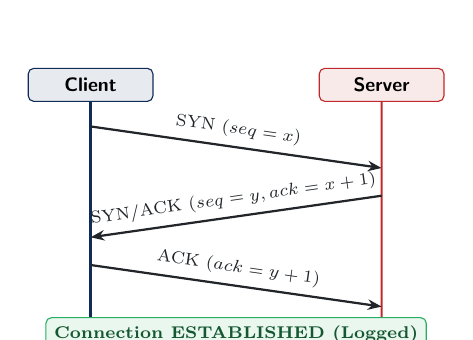
\begin{tikzpicture}[font=\sffamily\small, scale=0.88, every node/.style={transform shape}]
    \node[draw=primary, fill=primary!10, rounded corners=2pt, font=\sffamily\bfseries\footnotesize, inner sep=4pt, minimum width=1.8cm] (c) at (0, 0) {Client};
    \node[draw=alertred, fill=alertred!10, rounded corners=2pt, font=\sffamily\bfseries\footnotesize, inner sep=4pt, minimum width=1.8cm] (s) at (4.2, 0) {Server};
    
    \draw[thick, color=primary] (c.south) -- (0, -3.8);
    \draw[thick, color=alertred] (s.south) -- (4.2, -3.8);
    
    \draw[-{Stealth[length=5pt]}, thick, color=darkslate] (0, -0.6) -- node[above, sloped, font=\scriptsize] {SYN ($seq = x$)} (4.2, -1.2);
    \draw[-{Stealth[length=5pt]}, thick, color=darkslate] (4.2, -1.6) -- node[above, sloped, font=\scriptsize] {SYN/ACK ($seq = y, ack = x+1$)} (0, -2.2);
    \draw[-{Stealth[length=5pt]}, thick, color=darkslate] (0, -2.6) -- node[above, sloped, font=\scriptsize] {ACK ($ack = y+1$)} (4.2, -3.2);
    
    \node[draw=successgreen, fill=successgreen!10, rounded corners=2pt, font=\scriptsize\bfseries, align=center, text=successgreen!50!black] at (2.1, -3.6) {Connection ESTABLISHED (Logged)};
\end{tikzpicture}
\end{minipage}%
\hfill
\begin{minipage}[t]{0.485\textwidth}
\centering
{\color{primary}\sffamily\bfseries\small (b) Half-Open SYN Scan: Open Port}\\[6pt]
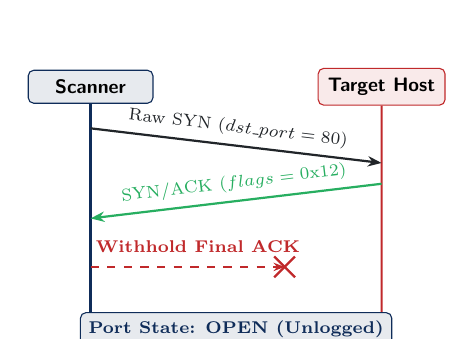
\begin{tikzpicture}[font=\sffamily\small, scale=0.88, every node/.style={transform shape}]
    \node[draw=primary, fill=primary!10, rounded corners=2pt, font=\sffamily\bfseries\footnotesize, inner sep=4pt, minimum width=1.8cm] (sc) at (0, 0) {Scanner};
    \node[draw=alertred, fill=alertred!10, rounded corners=2pt, font=\sffamily\bfseries\footnotesize, inner sep=4pt, minimum width=1.8cm] (th) at (4.2, 0) {Target Host};
    
    \draw[thick, color=primary] (sc.south) -- (0, -3.8);
    \draw[thick, color=alertred] (th.south) -- (4.2, -3.8);
    
    \draw[-{Stealth[length=5pt]}, thick, color=darkslate] (0, -0.6) -- node[above, sloped, font=\scriptsize] {Raw SYN ($dst\_port = 80$)} (4.2, -1.1);
    \draw[-{Stealth[length=5pt]}, thick, color=successgreen] (4.2, -1.4) -- node[above, sloped, font=\scriptsize] {SYN/ACK ($flags = \text{0x12}$)} (0, -1.9);
    
    \draw[-{Stealth[length=4pt]}, thick, dashed, color=alertred] (0, -2.6) -- (2.8, -2.6);
    \draw[thick, color=alertred] (2.65, -2.45) -- (2.95, -2.75);
    \draw[thick, color=alertred] (2.65, -2.75) -- (2.95, -2.45);
    \node[above=1pt, font=\scriptsize\color{alertred}\bfseries] at (1.55, -2.55) {Withhold Final ACK};
    
    \node[draw=primary, fill=primary!10, rounded corners=2pt, font=\scriptsize\bfseries, align=center, text=primary] at (2.1, -3.5) {Port State: \textbf{OPEN} (Unlogged)};
\end{tikzpicture}
\end{minipage}

\vspace{12pt}

\begin{minipage}[t]{0.485\textwidth}
\centering
{\color{primary}\sffamily\bfseries\small (c) Half-Open SYN Scan: Closed Port}\\[6pt]
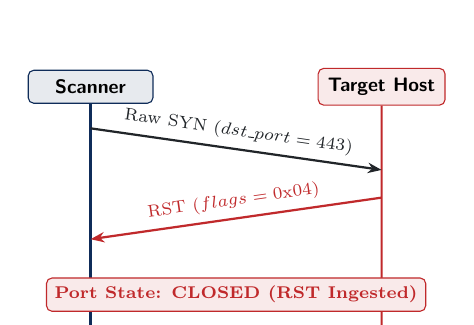
\begin{tikzpicture}[font=\sffamily\small, scale=0.88, every node/.style={transform shape}]
    \node[draw=primary, fill=primary!10, rounded corners=2pt, font=\sffamily\bfseries\footnotesize, inner sep=4pt, minimum width=1.8cm] (sc) at (0, 0) {Scanner};
    \node[draw=alertred, fill=alertred!10, rounded corners=2pt, font=\sffamily\bfseries\footnotesize, inner sep=4pt, minimum width=1.8cm] (th) at (4.2, 0) {Target Host};
    
    \draw[thick, color=primary] (sc.south) -- (0, -3.6);
    \draw[thick, color=alertred] (th.south) -- (4.2, -3.6);
    
    \draw[-{Stealth[length=5pt]}, thick, color=darkslate] (0, -0.6) -- node[above, sloped, font=\scriptsize] {Raw SYN ($dst\_port = 443$)} (4.2, -1.2);
    \draw[-{Stealth[length=5pt]}, thick, color=alertred] (4.2, -1.6) -- node[above, sloped, font=\scriptsize] {RST ($flags = \text{0x04}$)} (0, -2.2);
    
    \node[draw=alertred, fill=alertred!10, rounded corners=2pt, font=\scriptsize\bfseries, align=center, text=alertred] at (2.1, -3.0) {Port State: \textbf{CLOSED} (RST Ingested)};
\end{tikzpicture}
\end{minipage}%
\hfill
\begin{minipage}[t]{0.485\textwidth}
\centering
{\color{primary}\sffamily\bfseries\small (d) Half-Open SYN Scan: Filtered Port}\\[6pt]
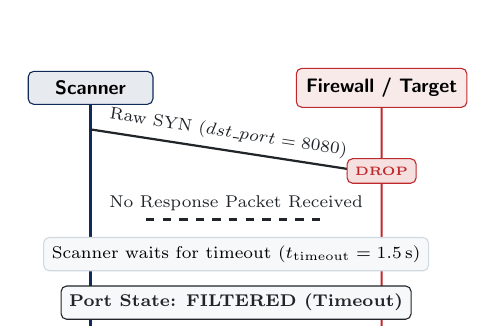
\begin{tikzpicture}[font=\sffamily\small, scale=0.88, every node/.style={transform shape}]
    \node[draw=primary, fill=primary!10, rounded corners=2pt, font=\sffamily\bfseries\footnotesize, inner sep=4pt, minimum width=1.8cm] (sc) at (0, 0) {Scanner};
    \node[draw=alertred, fill=alertred!10, rounded corners=2pt, font=\sffamily\bfseries\footnotesize, inner sep=4pt, minimum width=1.8cm] (th) at (4.2, 0) {Firewall / Target};
    
    \draw[thick, color=primary] (sc.south) -- (0, -3.6);
    \draw[thick, color=alertred] (th.south) -- (4.2, -3.6);
    
    \draw[-{Stealth[length=5pt]}, thick, color=darkslate] (0, -0.6) -- node[above, sloped, font=\scriptsize] {Raw SYN ($dst\_port = 8080$)} (3.9, -1.2);
    \node[draw=alertred, fill=alertred!15, rounded corners=2pt, font=\tiny\bfseries, text=alertred] at (4.2, -1.2) {DROP};
    
    \draw[thick, dashed, color=darkslate] (0.8, -1.9) -- (3.4, -1.9) 
        node[midway, above, font=\scriptsize\color{darkslate}] {No Response Packet Received};
    \node[draw=frameborder, fill=lightbg, rounded corners=2pt, font=\scriptsize, align=center] at (2.1, -2.4) {Scanner waits for timeout ($t_{\text{timeout}} = 1.5\,\text{s}$)};
    
    \node[draw=darkslate, fill=lightbg, rounded corners=2pt, font=\scriptsize\bfseries, align=center, text=darkslate] at (2.1, -3.1) {Port State: \textbf{FILTERED} (Timeout)};
\end{tikzpicture}
\end{minipage}
\caption{Protocol Timing Diagrams Comparing Standard TCP Handshake with Scanner Probe Classifications}
\label{fig:timing_scan}
\end{figure}

\subsection{Service Banner Grabbing Timing Sequences}
Banner grabbing extracts identification strings from services running on open ports. As shown in Figure~\ref{fig:timing_banner}, banner grabbing follows two patterns depending on whether the target service is passive or active:
\begin{itemize}
    \item \textbf{Passive Services (e.g., FTP, SMTP):} The listening daemon transmits an informational greeting banner immediately upon completion of the initial TCP 3-way handshake. The grabber establishes a standard connection, reads the incoming buffer, and terminates cleanly.
    \item \textbf{Active Services (HTTP):} Web daemons do not output unprompted greetings. The grabber establishes a connection, issues a minimal RFC-compliant probe (\texttt{HEAD / HTTP/1.0\textbackslash r\textbackslash n\textbackslash r\textbackslash n}), and extracts the software identification from the HTTP \texttt{Server:} header.
\end{itemize}

\begin{figure}[ht]
\centering
\begin{minipage}[t]{0.485\textwidth}
\centering
{\color{primary}\sffamily\bfseries\small (a) Passive Service Banner: FTP (Port 21)}\\[6pt]
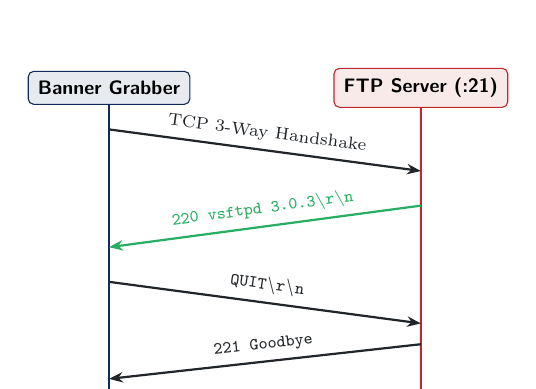
\begin{tikzpicture}[font=\sffamily\small, scale=0.88, every node/.style={transform shape}]
    \node[draw=primary, fill=primary!10, rounded corners=2pt, font=\sffamily\bfseries\footnotesize, inner sep=4pt, minimum width=2.2cm] (g) at (0, 0) {Banner Grabber};
    \node[draw=alertred, fill=alertred!10, rounded corners=2pt, font=\sffamily\bfseries\footnotesize, inner sep=4pt, minimum width=2.2cm] (s) at (4.5, 0) {FTP Server (:21)};
    
    \draw[thick, color=primary] (g.south) -- (0, -4.5);
    \draw[thick, color=alertred] (s.south) -- (4.5, -4.5);
    
    \draw[-{Stealth[length=5pt]}, thick, color=darkslate] (0, -0.6) -- node[above, sloped, font=\scriptsize] {TCP 3-Way Handshake} (4.5, -1.2);
    \draw[-{Stealth[length=5pt]}, thick, color=successgreen] (4.5, -1.7) -- node[above, sloped, font=\scriptsize\ttfamily] {220 vsftpd 3.0.3\textbackslash r\textbackslash n} (0, -2.3);
    \draw[-{Stealth[length=5pt]}, thick, color=darkslate] (0, -2.8) -- node[above, sloped, font=\scriptsize\ttfamily] {QUIT\textbackslash r\textbackslash n} (4.5, -3.4);
    \draw[-{Stealth[length=5pt]}, thick, color=darkslate] (4.5, -3.7) -- node[above, sloped, font=\scriptsize\ttfamily] {221 Goodbye} (0, -4.2);
\end{tikzpicture}
\end{minipage}%
\hfill
\begin{minipage}[t]{0.485\textwidth}
\centering
{\color{primary}\sffamily\bfseries\small (b) Active Service Banner: HTTP (Port 80)}\\[6pt]
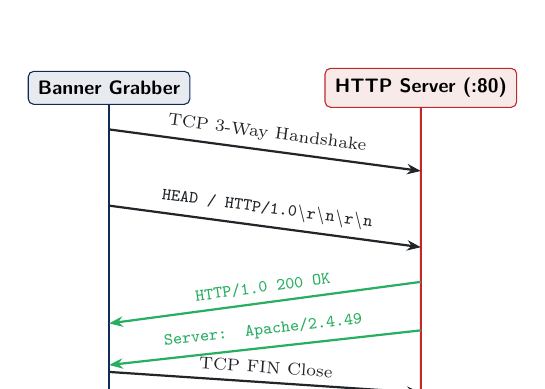
\begin{tikzpicture}[font=\sffamily\small, scale=0.88, every node/.style={transform shape}]
    \node[draw=primary, fill=primary!10, rounded corners=2pt, font=\sffamily\bfseries\footnotesize, inner sep=4pt, minimum width=2.2cm] (g) at (0, 0) {Banner Grabber};
    \node[draw=alertred, fill=alertred!10, rounded corners=2pt, font=\sffamily\bfseries\footnotesize, inner sep=4pt, minimum width=2.2cm] (s) at (4.5, 0) {HTTP Server (:80)};
    
    \draw[thick, color=primary] (g.south) -- (0, -4.5);
    \draw[thick, color=alertred] (s.south) -- (4.5, -4.5);
    
    \draw[-{Stealth[length=5pt]}, thick, color=darkslate] (0, -0.6) -- node[above, sloped, font=\scriptsize] {TCP 3-Way Handshake} (4.5, -1.2);
    \draw[-{Stealth[length=5pt]}, thick, color=darkslate] (0, -1.7) -- node[above, sloped, font=\scriptsize\ttfamily] {HEAD / HTTP/1.0\textbackslash r\textbackslash n\textbackslash r\textbackslash n} (4.5, -2.3);
    \draw[-{Stealth[length=5pt]}, thick, color=successgreen] (4.5, -2.8) -- node[above, sloped, font=\scriptsize\ttfamily] {HTTP/1.0 200 OK} (0, -3.4);
    \draw[-{Stealth[length=5pt]}, thick, color=successgreen] (4.5, -3.5) -- node[above, sloped, font=\scriptsize\ttfamily] {Server: Apache/2.4.49} (0, -4.0);
    \draw[-{Stealth[length=5pt]}, thick, color=darkslate] (0, -4.1) -- node[above, sloped, font=\scriptsize] {TCP FIN Close} (4.5, -4.4);
\end{tikzpicture}
\end{minipage}
\caption{Timing Sequences for Passive Banner Capture and Active Application Probing}
\label{fig:timing_banner}
\end{figure}

\subsection{Targeted Exploit Execution Timing}
After cataloging open ports and daemon versions, the orchestrator runs the targeted exploit modules. Figure~\ref{fig:timing_exploits} outlines the message sequences for anonymous FTP data access and HTTP path traversal.

\begin{figure}[ht]
\centering
\begin{minipage}[t]{0.485\textwidth}
\centering
{\color{primary}\sffamily\bfseries\small (a) Exploit 1: FTP Anonymous Access}\\[6pt]
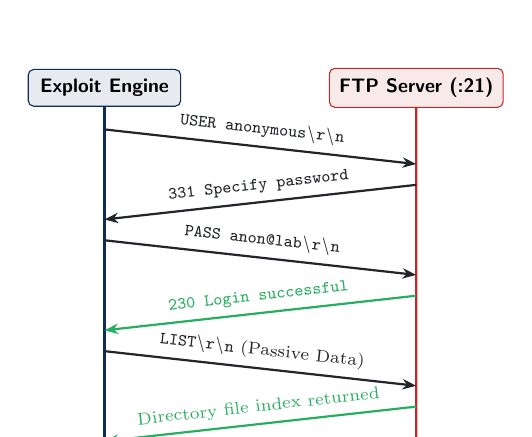
\begin{tikzpicture}[font=\sffamily\small, scale=0.88, every node/.style={transform shape}]
    \node[draw=primary, fill=primary!10, rounded corners=2pt, font=\sffamily\bfseries\footnotesize, inner sep=4pt, minimum width=2.2cm] (e) at (0, 0) {Exploit Engine};
    \node[draw=alertred, fill=alertred!10, rounded corners=2pt, font=\sffamily\bfseries\footnotesize, inner sep=4pt, minimum width=2.2cm] (s) at (4.5, 0) {FTP Server (:21)};
    
    \draw[thick, color=primary] (e.south) -- (0, -5.2);
    \draw[thick, color=alertred] (s.south) -- (4.5, -5.2);
    
    \draw[-{Stealth[length=5pt]}, thick, color=darkslate] (0, -0.6) -- node[above, sloped, font=\scriptsize\ttfamily] {USER anonymous\textbackslash r\textbackslash n} (4.5, -1.1);
    \draw[-{Stealth[length=5pt]}, thick, color=darkslate] (4.5, -1.4) -- node[above, sloped, font=\scriptsize\ttfamily] {331 Specify password} (0, -1.9);
    \draw[-{Stealth[length=5pt]}, thick, color=darkslate] (0, -2.2) -- node[above, sloped, font=\scriptsize\ttfamily] {PASS anon@lab\textbackslash r\textbackslash n} (4.5, -2.7);
    \draw[-{Stealth[length=5pt]}, thick, color=successgreen] (4.5, -3.0) -- node[above, sloped, font=\scriptsize\ttfamily] {230 Login successful} (0, -3.5);
    \draw[-{Stealth[length=5pt]}, thick, color=darkslate] (0, -3.8) -- node[above, sloped, font=\scriptsize] {\texttt{LIST\textbackslash r\textbackslash n} (Passive Data)} (4.5, -4.3);
    \draw[-{Stealth[length=5pt]}, thick, color=successgreen] (4.5, -4.6) -- node[above, sloped, font=\scriptsize] {Directory file index returned} (0, -5.1);
\end{tikzpicture}
\end{minipage}%
\hfill
\begin{minipage}[t]{0.485\textwidth}
\centering
{\color{primary}\sffamily\bfseries\small (b) Exploit 2: HTTP Directory Path Traversal}\\[6pt]
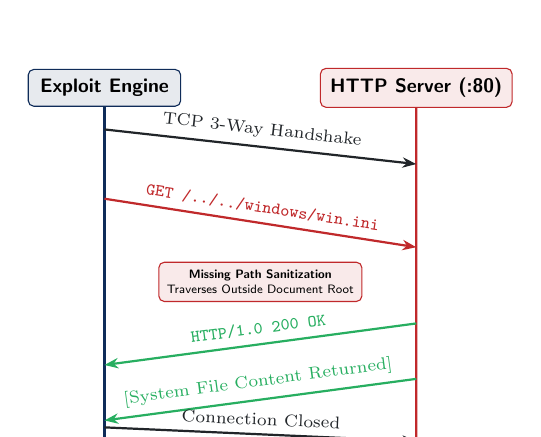
\begin{tikzpicture}[font=\sffamily\small, scale=0.88, every node/.style={transform shape}]
    \node[draw=primary, fill=primary!10, rounded corners=2pt, font=\sffamily\bfseries\footnotesize, inner sep=4pt, minimum width=2.2cm] (e) at (0, 0) {Exploit Engine};
    \node[draw=alertred, fill=alertred!10, rounded corners=2pt, font=\sffamily\bfseries\footnotesize, inner sep=4pt, minimum width=2.2cm] (s) at (4.5, 0) {HTTP Server (:80)};
    
    \draw[thick, color=primary] (e.south) -- (0, -5.2);
    \draw[thick, color=alertred] (s.south) -- (4.5, -5.2);
    
    \draw[-{Stealth[length=5pt]}, thick, color=darkslate] (0, -0.6) -- node[above, sloped, font=\scriptsize] {TCP 3-Way Handshake} (4.5, -1.1);
    \draw[-{Stealth[length=5pt]}, thick, color=alertred] (0, -1.6) -- node[above, sloped, font=\scriptsize\ttfamily] {GET /../../windows/win.ini} (4.5, -2.3);
    
    % Centered callout box
    \node[draw=alertred, fill=alertred!10, rounded corners=2pt, font=\tiny\sffamily, align=center] at (2.25, -2.8) {
        \textbf{Missing Path Sanitization}\\Traverses Outside Document Root
    };
    
    \draw[-{Stealth[length=5pt]}, thick, color=successgreen] (4.5, -3.4) -- node[above, sloped, font=\scriptsize\ttfamily] {HTTP/1.0 200 OK} (0, -4.0);
    \draw[-{Stealth[length=5pt]}, thick, color=successgreen] (4.5, -4.2) -- node[above, sloped, font=\scriptsize] {[System File Content Returned]} (0, -4.8);
    \draw[-{Stealth[length=5pt]}, thick, color=darkslate] (0, -4.9) -- node[above, sloped, font=\scriptsize] {Connection Closed} (4.5, -5.1);
\end{tikzpicture}
\end{minipage}
\caption{Protocol Interactions Demonstrating Concrete Exploit Outcomes}
\label{fig:timing_exploits}
\end{figure}

\subsection{Defense Detection and Mitigation Timeline}
Figure~\ref{fig:timing_defense} shows the defense monitor timeline. Incoming SYN packets update a sliding-window queue on the target host. When probe volume reaches 8 SYN packets across at least 5 distinct ports within 10 seconds, the monitor triggers an alert and adds an inbound firewall rule blocking the scanner's IP. The network interface drops subsequent probes before they reach application sockets.

\begin{figure}[ht]
\centering
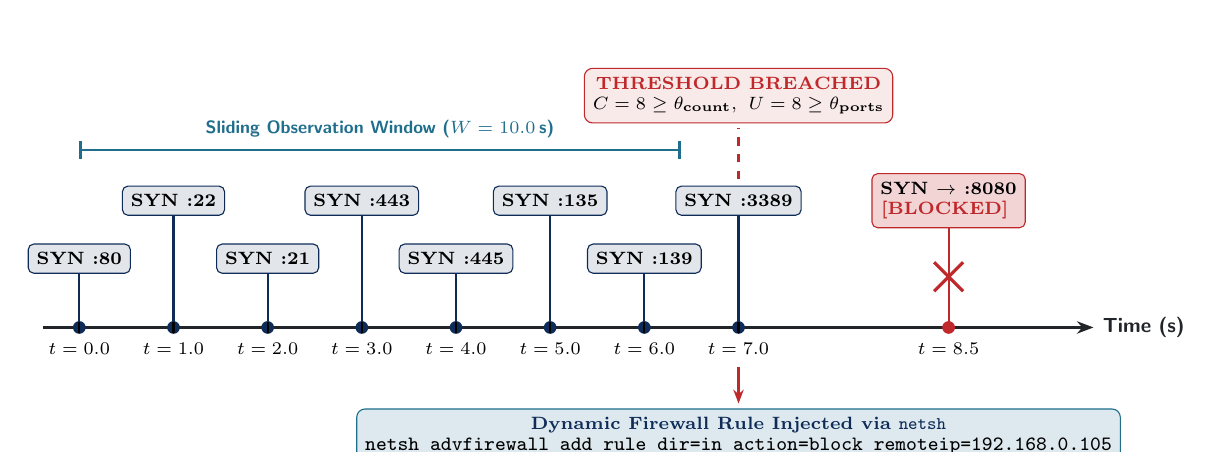
\begin{tikzpicture}[
    font=\sffamily\small,
    scale=0.92, every node/.style={transform shape}
]
    % ------------------------------------------------------------------
    % Time Axis
    % ------------------------------------------------------------------
    \draw[thick, -{Stealth[length=6pt]}, color=darkslate] (0, 0) -- (14.5, 0) node[right, font=\sffamily\footnotesize\bfseries] {Time (s)};
    
    % ------------------------------------------------------------------
    % Sliding Observation Window Indicator Bar
    % ------------------------------------------------------------------
    \draw[secondary, thick, |-|] (0.5, 2.45) -- (8.8, 2.45) 
        node[midway, above=1pt, font=\sffamily\scriptsize\bfseries, color=secondary] {Sliding Observation Window ($W = 10.0\,\text{s}$)};

    % ------------------------------------------------------------------
    % Staggered SYN Probe Impulses (Alternating Heights: 0.75 and 1.55)
    % ------------------------------------------------------------------
    % 1: t=0.0 (x=0.5)
    \draw[thick, color=primary] (0.5, 0) -- (0.5, 0.75);
    \fill[primary] (0.5, 0) circle (2.5pt);
    \node[draw=primary, fill=primary!12, rounded corners=2pt, font=\scriptsize\bfseries] at (0.5, 0.95) {SYN :80};

    % 2: t=1.0 (x=1.8)
    \draw[thick, color=primary] (1.8, 0) -- (1.8, 1.55);
    \fill[primary] (1.8, 0) circle (2.5pt);
    \node[draw=primary, fill=primary!12, rounded corners=2pt, font=\scriptsize\bfseries] at (1.8, 1.75) {SYN :22};

    % 3: t=2.0 (x=3.1)
    \draw[thick, color=primary] (3.1, 0) -- (3.1, 0.75);
    \fill[primary] (3.1, 0) circle (2.5pt);
    \node[draw=primary, fill=primary!12, rounded corners=2pt, font=\scriptsize\bfseries] at (3.1, 0.95) {SYN :21};

    % 4: t=3.0 (x=4.4)
    \draw[thick, color=primary] (4.4, 0) -- (4.4, 1.55);
    \fill[primary] (4.4, 0) circle (2.5pt);
    \node[draw=primary, fill=primary!12, rounded corners=2pt, font=\scriptsize\bfseries] at (4.4, 1.75) {SYN :443};

    % 5: t=4.0 (x=5.7)
    \draw[thick, color=primary] (5.7, 0) -- (5.7, 0.75);
    \fill[primary] (5.7, 0) circle (2.5pt);
    \node[draw=primary, fill=primary!12, rounded corners=2pt, font=\scriptsize\bfseries] at (5.7, 0.95) {SYN :445};

    % 6: t=5.0 (x=7.0)
    \draw[thick, color=primary] (7.0, 0) -- (7.0, 1.55);
    \fill[primary] (7.0, 0) circle (2.5pt);
    \node[draw=primary, fill=primary!12, rounded corners=2pt, font=\scriptsize\bfseries] at (7.0, 1.75) {SYN :135};

    % 7: t=6.0 (x=8.3)
    \draw[thick, color=primary] (8.3, 0) -- (8.3, 0.75);
    \fill[primary] (8.3, 0) circle (2.5pt);
    \node[draw=primary, fill=primary!12, rounded corners=2pt, font=\scriptsize\bfseries] at (8.3, 0.95) {SYN :139};

    % 8: t=7.0 (x=9.6) - THRESHOLD BREACH!
    \draw[thick, color=primary] (9.6, 0) -- (9.6, 1.55);
    \fill[primary] (9.6, 0) circle (2.5pt);
    \node[draw=primary, fill=primary!12, rounded corners=2pt, font=\scriptsize\bfseries] at (9.6, 1.75) {SYN :3389};

    % ------------------------------------------------------------------
    % Axis Ticks and Time Labels
    % ------------------------------------------------------------------
    \foreach \x/\timeval in {0.5/0.0, 1.8/1.0, 3.1/2.0, 4.4/3.0, 5.7/4.0, 7.0/5.0, 8.3/6.0, 9.6/7.0, 12.5/8.5} {
        \draw[thick] (\x, 0.08) -- (\x, -0.08) node[below=2pt, font=\scriptsize, fill=white, inner sep=1.5pt] {$t=\timeval$};
    }

    % ------------------------------------------------------------------
    % Vertical Threshold Trigger Line and Badge (cleanly outside probe box)
    % ------------------------------------------------------------------
    \draw[thick, dashed, color=alertred] (9.6, 2.05) -- (9.6, 2.75);
    \node[draw=alertred, fill=alertred!10, rounded corners=3pt, font=\scriptsize\bfseries, align=center] at (9.6, 3.2) {
        \color{alertred}\textbf{THRESHOLD BREACHED}\\
        \scriptsize $C = 8 \ge \theta_{\text{count}}, \ U = 8 \ge \theta_{\text{ports}}$
    };

    % ------------------------------------------------------------------
    % Firewall Mitigation Callout Below Axis
    % ------------------------------------------------------------------
    \draw[-{Stealth[length=5pt]}, thick, color=alertred] (9.6, -0.55) -- (9.6, -1.05);
    \node[draw=secondary, fill=secondary!15, rounded corners=3pt, font=\scriptsize, align=center] at (9.6, -1.5) {
        \textbf{\color{primary}Dynamic Firewall Rule Injected via \texttt{netsh}}\\
        \texttt{\footnotesize netsh advfirewall add rule dir=in action=block remoteip=192.168.0.105}
    };

    % ------------------------------------------------------------------
    % Blocked 9th Probe at t=8.5 (x=12.5)
    % ------------------------------------------------------------------
    \draw[thick, color=alertred] (12.5, 0) -- (12.5, 1.4);
    \fill[alertred] (12.5, 0) circle (2.5pt);
    \node[draw=alertred, fill=alertred!20, rounded corners=2pt, font=\scriptsize\bfseries, align=center] at (12.5, 1.75) {
        SYN $\to$ :8080\\
        \color{alertred}\textbf{[BLOCKED]}
    };
    % Cross marker
    \draw[line width=1.2pt, color=alertred] (12.3, 0.5) -- (12.7, 0.9);
    \draw[line width=1.2pt, color=alertred] (12.3, 0.9) -- (12.7, 0.5);

\end{tikzpicture}
\caption{Timeline of Sliding-Window Scan Detection and Dynamic Firewall Rule Injection}
\label{fig:timing_defense}
\end{figure}

% ----------------------------------------------------------------------
% 4. Packet and Frame Structure
% ----------------------------------------------------------------------
\section{Binary Packet and Frame Structure}

\subsection{Layer 2: Ethernet II Frame Header}
Every transmitted probe is encapsulated in an Ethernet II frame consisting of 14 header octets:

\begin{figure}[ht]
\centering
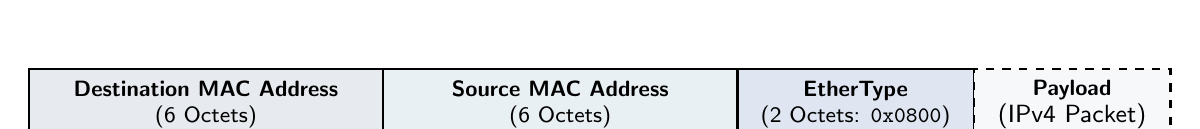
\begin{tikzpicture}[font=\sffamily\footnotesize]
    \draw[thick, fill=primary!10] (0, 0) rectangle (4.5, 0.9) node[midway, align=center] {\textbf{Destination MAC Address}\\(6 Octets)};
    \draw[thick, fill=secondary!10] (4.5, 0) rectangle (9.0, 0.9) node[midway, align=center] {\textbf{Source MAC Address}\\(6 Octets)};
    \draw[thick, fill=accent!15] (9.0, 0) rectangle (12.0, 0.9) node[midway, align=center] {\textbf{EtherType}\\(2 Octets: \texttt{0x0800})};
    \draw[thick, fill=lightbg, dashed] (12.0, 0) rectangle (14.5, 0.9) node[midway, align=center] {\textbf{Payload}\\\small(IPv4 Packet)};
\end{tikzpicture}
\caption{Layer 2 Ethernet II Frame Structure (Total Header: 14 Octets)}
\label{fig:frame_eth}
\end{figure}

\subsection{Layer 3: IPv4 Packet Header}
The IPv4 packet is constructed strictly according to RFC 791. Standard probes use a 20-byte base header without IP options:

\begin{figure}[ht]
\centering
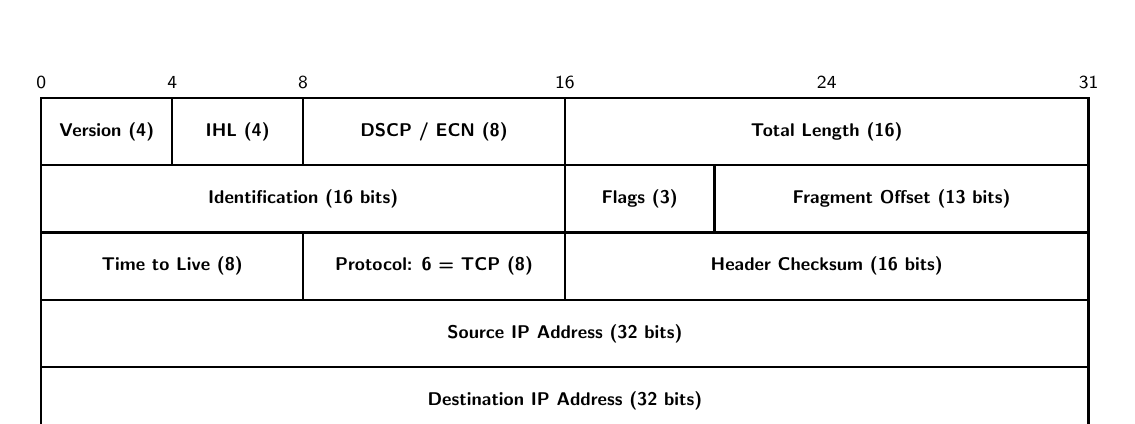
\begin{tikzpicture}[scale=0.95, every node/.style={transform shape}, font=\sffamily\scriptsize]
    % Header bit scale (0 to 31)
    \draw[thick] (0, 4.5) rectangle (14, 0);
    
    % Bit labels
    \node[above] at (0, 4.5) {0};
    \node[above] at (1.75, 4.5) {4};
    \node[above] at (3.5, 4.5) {8};
    \node[above] at (7.0, 4.5) {16};
    \node[above] at (10.5, 4.5) {24};
    \node[above] at (14, 4.5) {31};

    % Row 1: Version, IHL, DSCP/ECN, Total Length
    \draw[thick] (0, 3.6) -- (14, 3.6);
    \draw[thick] (1.75, 4.5) -- (1.75, 3.6);
    \draw[thick] (3.5, 4.5) -- (3.5, 3.6);
    \draw[thick] (7.0, 4.5) -- (7.0, 3.6);
    \node at (0.875, 4.05) {\textbf{Version (4)}};
    \node at (2.625, 4.05) {\textbf{IHL (4)}};
    \node at (5.25, 4.05) {\textbf{DSCP / ECN (8)}};
    \node at (10.5, 4.05) {\textbf{Total Length (16)}};

    % Row 2: Identification, Flags, Fragment Offset
    \draw[thick] (0, 2.7) -- (14, 2.7);
    \draw[thick] (7.0, 3.6) -- (7.0, 2.7);
    \draw[thick] (9.0, 3.6) -- (9.0, 2.7);
    \node at (3.5, 3.15) {\textbf{Identification (16 bits)}};
    \node at (8.0, 3.15) {\textbf{Flags (3)}};
    \node at (11.5, 3.15) {\textbf{Fragment Offset (13 bits)}};

    % Row 3: TTL, Protocol, Header Checksum
    \draw[thick] (0, 1.8) -- (14, 1.8);
    \draw[thick] (3.5, 2.7) -- (3.5, 1.8);
    \draw[thick] (7.0, 2.7) -- (7.0, 1.8);
    \node at (1.75, 2.25) {\textbf{Time to Live (8)}};
    \node at (5.25, 2.25) {\textbf{Protocol: 6 = TCP (8)}};
    \node at (10.5, 2.25) {\textbf{Header Checksum (16 bits)}};

    % Row 4: Source IP
    \draw[thick] (0, 0.9) -- (14, 0.9);
    \node at (7.0, 1.35) {\textbf{Source IP Address (32 bits)}};

    % Row 5: Destination IP
    \node at (7.0, 0.45) {\textbf{Destination IP Address (32 bits)}};
\end{tikzpicture}
\caption{Layer 3 IPv4 Packet Header Format (20 Octets Base)}
\label{fig:header_ipv4}
\end{figure}

\subsection{Layer 4: TCP Segment Header and Active Option Offering}
The TCP header is serialized per RFC 793 with control flags explicitly set for the SYN half-open probe ($Flags = \text{0x02}$). While a minimal TCP header spans 20 octets ($\text{Data Offset} = 5$), standard probes in our proposed toolkit are structured as 40-octet frames ($\text{Data Offset} = 10$) incorporating 20 octets of diagnostic TCP options (\texttt{STANDARD\_SYN\_OPTIONS}):
\begin{itemize}[nosep, leftmargin=1.5em]
    \item \textbf{Maximum Segment Size (MSS):} Option Kind 2, Length 4, Value $1460$ (\texttt{0x02 0x04 0x05 0xb4}).
    \item \textbf{SACK Permitted:} Option Kind 4, Length 2 (\texttt{0x04 0x02}), advertising RFC~2018 selective acknowledgment support.
    \item \textbf{TCP Timestamp:} Option Kind 8, Length 10 (\texttt{0x08 0x0a ...}), advertising RFC~7323 timestamp capabilities.
    \item \textbf{Window Scale:} Option Kind 3, Length 3, Shift count $8$ (\texttt{0x03 0x03 0x08}), padded with a NOP (\texttt{0x01}) for 32-bit boundary alignment.
\end{itemize}
Offering these options prompts the target host to negotiate and reveal its native TCP option order, window scale factor, and timestamp support in the SYN/ACK reply.

\subsubsection{Active Stimulus-Response TCP Option Formulation}
Under RFC 7323 (TCP High Performance Extensions) and RFC 2018 (Selective Acknowledgment), advanced TCP capabilities require mutual negotiation during the initial handshake. If a scanner sends a bare 20-byte TCP SYN header without options, target operating systems omit Window Scale, SACK-Permitted, and Timestamp fields in their SYN/ACK replies.

Our probe design addresses this by including an active option stimulus in every outgoing SYN packet:
\begin{equation}
\text{SYN}_{\text{options}} = \langle \text{MSS}(1460), \ \text{SACK\_PERMITTED}, \ \text{TIMESTAMP}(t_0, 0), \ \text{NOP}, \ \text{WSCALE}(8) \rangle
\end{equation}
Offering these capabilities prompts the target kernel to return its full set of negotiated parameters:
\begin{itemize}[nosep, leftmargin=1.4em]
    \item The compile-time \textbf{option sequence order}, which varies by vendor (for example, Apple Darwin stacks place Window Scale before Timestamp, while Linux stacks place SACK-Permitted before Timestamp).
    \item The native \textbf{Window Scale factor} ($S \in \{5, 6, 7, 8\}$).
    \item Adherence to RFC 6864, which determines whether the target clears the IPv4 Identification field on atomic datagrams.
\end{itemize}

The base 20-octet header structure is shown in Figure~\ref{fig:header_tcp}:

\begin{figure}[ht]
\centering
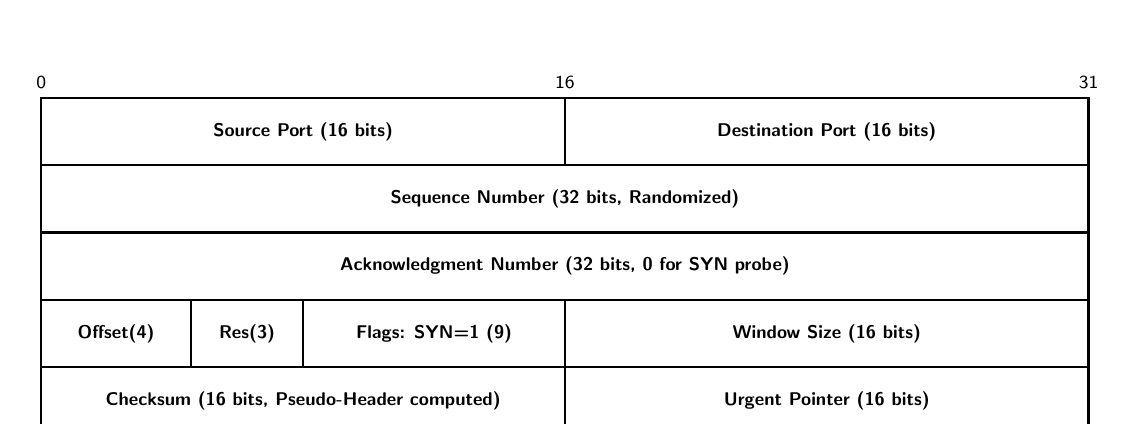
\begin{tikzpicture}[scale=0.95, every node/.style={transform shape}, font=\sffamily\scriptsize]
    \draw[thick] (0, 4.5) rectangle (14, 0);

    % Bit labels
    \node[above] at (0, 4.5) {0};
    \node[above] at (7.0, 4.5) {16};
    \node[above] at (14, 4.5) {31};

    % Row 1: Source and Destination Ports
    \draw[thick] (0, 3.6) -- (14, 3.6);
    \draw[thick] (7.0, 4.5) -- (7.0, 3.6);
    \node at (3.5, 4.05) {\textbf{Source Port (16 bits)}};
    \node at (10.5, 4.05) {\textbf{Destination Port (16 bits)}};

    % Row 2: Sequence Number
    \draw[thick] (0, 2.7) -- (14, 2.7);
    \node at (7.0, 3.15) {\textbf{Sequence Number (32 bits, Randomized)}};

    % Row 3: Acknowledgment Number
    \draw[thick] (0, 1.8) -- (14, 1.8);
    \node at (7.0, 2.25) {\textbf{Acknowledgment Number (32 bits, 0 for SYN probe)}};

    % Row 4: Data Offset, Reserved, Flags, Window Size
    \draw[thick] (0, 0.9) -- (14, 0.9);
    \draw[thick] (2.0, 1.8) -- (2.0, 0.9);
    \draw[thick] (3.5, 1.8) -- (3.5, 0.9);
    \draw[thick] (7.0, 1.8) -- (7.0, 0.9);
    \node at (1.0, 1.35) {\textbf{Offset(4)}};
    \node at (2.75, 1.35) {\textbf{Res(3)}};
    \node at (5.25, 1.35) {\textbf{Flags: SYN=1 (9)}};
    \node at (10.5, 1.35) {\textbf{Window Size (16 bits)}};

    % Row 5: Checksum, Urgent Pointer
    \draw[thick] (7.0, 0.9) -- (7.0, 0);
    \node at (3.5, 0.45) {\textbf{Checksum (16 bits, Pseudo-Header computed)}};
    \node at (10.5, 0.45) {\textbf{Urgent Pointer (16 bits)}};
\end{tikzpicture}
\caption{Layer 4 TCP Segment Header Format (20 Octets Base)}
\label{fig:header_tcp}
\end{figure}

\subsection{TCP Checksum Calculation and Pseudo-Header Construction}
Under RFC 793, the TCP checksum is not calculated over the TCP segment alone. It covers a 12-byte pseudo-header prepended to the TCP segment to verify that the packet reached its intended destination IP address:

\begin{equation}
\text{Checksum} = \sim \left( \sum_{i=1}^{N} W_i \pmod{2^{16} - 1} \right)
\end{equation}

where $W_i$ represents consecutive 16-bit words across the concatenated pseudo-header and TCP segment. The pseudo-header structure is defined in Table~\ref{tab:pseudo_header}:

\begin{table}[ht]
\centering
\small
\renewcommand{\arraystretch}{1.25}
\caption{IPv4 TCP Pseudo-Header Field Layout for Checksum Calculation}
\label{tab:pseudo_header}
\begin{tabularx}{\textwidth}{>{\raggedright\arraybackslash\bfseries}p{2.6cm} >{\raggedright\arraybackslash}p{4.8cm} >{\raggedright\arraybackslash}X}
\toprule
\textbf{Byte Offset} & \textbf{Field Name} & \textbf{Value in SYN Probe} \\
\midrule
0--3  & Source IPv4 Address      & Attacker IPv4 (e.g., \texttt{192.168.0.105}) \\
4--7  & Destination IPv4 Address & Target IPv4 (e.g., \texttt{192.168.0.116}) \\
8     & Reserved Zero Octet      & \texttt{0x00} \\
9     & Protocol Identifier      & \texttt{0x06} (TCP Transport Protocol) \\
10--11& TCP Segment Length       & Length of TCP header + options + payload (e.g., 20) \\
\bottomrule
\end{tabularx}
\end{table}

\subsection{OS Fingerprinting Diagnostic Signature Matrix}
The fingerprinting engine parses incoming response frames (open-port SYN/ACKs or closed-port RSTs) and extracts diagnostic attributes across Layer~3 and Layer~4 headers. Table~\ref{tab:fingerprint_matrix} defines the baseline signature matrix across target operating system families:

\begin{table}[ht]
\centering
\footnotesize
\renewcommand{\arraystretch}{1.22}
\caption{TCP/IP Stack Fingerprinting Signatures across Operating System Families}
\label{tab:fingerprint_matrix}
\begin{tabularx}{\textwidth}{>{\raggedright\arraybackslash\bfseries}p{3.0cm} >{\raggedright\arraybackslash}p{2.2cm} >{\centering\arraybackslash}X >{\centering\arraybackslash}X >{\centering\arraybackslash}X >{\centering\arraybackslash}X}
\toprule
\textbf{Diagnostic Feature} & \textbf{Protocol Field} & \textbf{Windows 10/11} & \textbf{Linux Modern} & \textbf{macOS / Modern BSD} & \textbf{Network Device} \\
\midrule
Initial TTL (SYN/ACK) & IPv4 TTL & 128 & 64 & 64 & 255 \\
\rowcolor{lightbg}
Don't Fragment (DF) & IPv4 Flags & Set & Set & Set & Often Clear \\
IPv4 ID (RFC 6864) & IPv4 ID & Non-Zero / Random & Strictly 0 (with DF) & Non-Zero / Sequential & Sequential \\
\rowcolor{lightbg}
Advertised Window & TCP Window & 64240, 65535, 8192 & 29200, 65160, 14600 & 65535, 33304 & 4128, 8192 \\
Window Scale Factor & TCP Option 3 & 8 & 7 or 8 & 5 or 6 & 0 or 2 \\
\rowcolor{lightbg}
TCP Timestamp & TCP Option 8 & Often Absent & Present & Present & Typically Absent \\
Option Sequence & TCP Options & M, W, S, T or M, W, S & M, S, T, W (SACK $<$ TS) & M, W, T, S (WS $<$ TS) & MSS Only / None \\
\rowcolor{lightbg}
Closed-Port RST TTL & IPv4 TTL (RST) & 128 & 64 & 64 & 255 \\
Closed-Port Window & TCP Window (RST) & 0 & 0 & 0 & 0 \\
\rowcolor{lightbg}
Closed-Port RST IP ID & IPv4 ID (RST) & Non-Zero & 0 (with DF set) & Non-Zero / DF Clear & Non-Zero \\
\bottomrule
\end{tabularx}
\end{table}

\subsection{Mathematical Formulation of Probabilistic OS Scoring and Version Tiering}
Passive operating system detection cannot rely on simple exact matches, because middleboxes and overlapping TCP window configurations often obscure single fields. The proposed engine formulates OS identification as a weighted evidence score across four classes: $\mathcal{C} = \{\text{Windows}, \text{Linux}, \text{macOS / BSD}, \text{Network device}\}$.

\subsubsection{Evidence-Based Scoring Model}
For an extracted feature set $F = \{\text{TTL}_{\text{obs}}, W_{\text{obs}}, \text{DF}, \text{ID}_{\text{obs}}, \text{Options}_{\text{order}}, \text{IsRST}\}$, the score $S_c$ for each class $c \in \mathcal{C}$ is computed as:
\begin{equation}
S_c = \sum_{k} w_{k,c} \cdot \phi_k(F, c)
\end{equation}
where $\phi_k(F, c) \in \{0, 1\}$ indicates whether observed feature $k$ satisfies the signature predicate for class $c$, and $w_{k,c} > 0$ represents diagnostic confidence weightings:
\begin{itemize}[nosep, leftmargin=1.4em]
    \item \textbf{Normalized Initial TTL ($w = +4.0$):} Observed TTL $T_{\text{obs}}$ is normalized to standard boundary $T_{\text{norm}} \in \{32, 64, 128, 255\}$ via $T_{\text{norm}} = \min \{t \in \{32, 64, 128, 255\} \mid t \ge T_{\text{obs}}\}$. Estimated router hops are $H = T_{\text{norm}} - T_{\text{obs}}$.
    \item \textbf{TCP Option Sequence Order ($w = +3.0$):} Option sequence order separates Linux from Darwin directly: Linux kernels place SACK-Permitted before Timestamp ($\langle\text{MSS}, \text{SACK}, \text{TS}, \text{WS}\rangle$), whereas Apple Darwin and BSD stacks place Window Scale before Timestamp ($\langle\text{MSS}, \text{WS}, \text{TS}, \text{SACK}\rangle$).
    \item \textbf{RFC 6864 IPv4 Identification ($w = +1.5$ / $+0.8$):} When DF is asserted, $\text{ID}_{\text{obs}} = 0$ provides $+1.5$ weight to Linux; non-zero ID awards $+0.8$ to Windows and $+0.4$ to macOS/BSD.
    \item \textbf{Closed-Port RST Ingestion ($w = +4.5$):} When zero ports are open, a returned RST with $T_{\text{norm}} = 128$ and $W_{\text{obs}} = 0$ awards $+4.5$ to Windows; $T_{\text{norm}} = 64$ awards $+3.0$ to Linux/BSD.
    \item \textbf{Advertised Window and Window Scale ($w = +1.5$ / $+1.0$):} Evaluates advertised window buffer presets and scale shift exponents against known vendor defaults.
\end{itemize}

The cumulative raw scores are normalized into a ranked probability distribution vector $\mathbf{P}$:
\begin{equation}
P(c) = \frac{\max(0, S_c)}{\sum_{j \in \mathcal{C}} \max(0, S_j)} \times 100\%, \quad \forall c \in \mathcal{C}
\end{equation}

\subsubsection{Hierarchical Version Tiering Model}
Because releases within the same operating system family share identical stack parameters, the design classifies targets into coarse family tiers using secondary feature checks:
\begin{itemize}[nosep, leftmargin=1.4em]
    \item \textbf{Windows Tiers:} Evaluates initial TTL 32 vs 128, timestamp absence, and legacy buffer sizes (8192 vs 65535) to discriminate between \textit{Windows 10 / 11 / Server 2016+}, \textit{Windows 7 / 8 / Vista}, and \textit{Legacy Windows 9x / 2000}.
    \item \textbf{Linux Tiers:} Differentiates \textit{Linux modern kernel (3.x / 4.x / 5.x+)} from \textit{Linux legacy (2.4 / 2.6)} based on RFC~6864 IP ID zeroing and modern window scaling presets.
    \item \textbf{macOS / BSD Tiers:} Classifies into \textit{macOS / modern BSD} (evaluating Darwin option ordering and window scale 5--6) versus \textit{Legacy BSD / NetBSD}.
\end{itemize}

% ----------------------------------------------------------------------
% 5. Implementation Plan and Modular Architecture
% ----------------------------------------------------------------------
\section{Implementation Plan and Modular Architecture}

\subsection{Modular Repository Architecture}
The project codebase is organized into four decoupled packages:

\begin{itemize}
    \item \textbf{\texttt{common/}:} Shared core networking utilities.
    \begin{itemize}
        \item \texttt{packet.py}: Implements \texttt{build\_syn\_frame()}, \texttt{parse\_ipv4\_tcp\_frame()}, and the RFC 1071 checksum routine.
        \item \texttt{npcap.py}: Provides native \texttt{ctypes} wrappers for \texttt{wpcap.dll} functions, including \texttt{pcap\_open}, \texttt{pcap\_sendpacket}, and \texttt{pcap\_next\_ex}.
    \end{itemize}
    \item \textbf{\texttt{attacker/}:} Multi-phase attack orchestration suite.
    \begin{itemize}
        \item \texttt{main.py}: Master CLI coordinator linking all reconnaissance and exploit phases.
        \item \texttt{scanner.py}: TCP SYN port scanner implementing the half-open probe loop.
        \item \texttt{banner.py}: Stream socket connection routines for passive and active banner extraction.
        \item \texttt{fingerprint.py}: Heuristic scorer comparing SYN/ACK attributes against known signatures.
        \item \texttt{exploits/}: Dedicated modules for anonymous FTP authentication and HTTP directory path traversal.
    \end{itemize}
    \item \textbf{\texttt{victim/}:} Reproducible demonstration targets.
    \begin{itemize}
        \item \texttt{ftp\_server.py}: Multithreaded Python FTP server configured to accept anonymous logins.
        \item \texttt{http\_server.py}: HTTP daemon containing an intentional path traversal flaw.
    \end{itemize}
    \item \textbf{\texttt{defense/}:} Countermeasure implementation.
    \begin{itemize}
        \item \texttt{detector.py}: In-memory sliding-window packet queue tracking per-IP probe frequency and destination port counts.
        \item \texttt{main.py}: Automated alert dispatcher executing \texttt{netsh advfirewall} commands to enforce temporary IP blocks.
    \end{itemize}
\end{itemize}

\subsection{Automated Verification and Unit Testing Framework}
To verify packet construction and scoring algorithms before physical network testing, the implementation plan includes an automated unit test suite built with \texttt{pytest}. The suite provides test coverage across two dedicated modules:

\begin{itemize}[nosep, itemsep=2pt, leftmargin=1.5em]
    \item \texttt{tests/test\_packet.py}:
    \begin{itemize}
        \item \textbf{RFC 1071 Checksum Verification:} Validates 16-bit one's complement addition over odd-length and even-length buffers against standard test vectors.
        \item \textbf{Binary Framing Roundtrip:} Confirms that serialized Ethernet, IPv4, and TCP frames unpack into their original field values without distortion.
        \item \textbf{TCP Option Parsing:} Tests parsing of option streams containing MSS, Window Scale, SACK-Permitted, and Timestamp fields with variable NOP padding.
    \end{itemize}
    \item \texttt{tests/test\_fingerprint.py}:
    \begin{itemize}
        \item \textbf{TTL Normalization and Hop Estimation:} Verifies rounding to standard boundaries (32, 64, 128, 255) across simulated network hops.
        \item \textbf{RFC 6864 IP ID Evaluation:} Confirms that datagrams with $\text{DF}=1$ and $\text{IP ID}=0$ correctly increase the Linux classification score.
        \item \textbf{Closed-Port RST Classification:} Tests that zero-window RST responses classify Windows targets accurately when no open ports exist.
        \item \textbf{Version Tiering Logic:} Verifies hierarchical scoring between legacy and modern Windows and Linux releases.
    \end{itemize}
\end{itemize}

% ----------------------------------------------------------------------
% 6. Justification: Why the Design Will Work
% ----------------------------------------------------------------------
\section{Justification and Technical Viability}

The technical approach relies on four standard protocol behaviors:
\begin{enumerate}[nosep, itemsep=3pt, leftmargin=1.4em]
    \item \textbf{Deterministic Kernel Responses (RFC 793 / RFC 9293):} Operating system kernels must reply with RST for packets to closed ports and SYN/ACK for active listening ports. Because these replies come directly from the kernel network stack, the scanner determines port states without establishing an application session, and ingests both SYN/ACK and RST frames for passive OS classification.
    \item \textbf{Link-Layer Transmission via Npcap:} Standard Windows sockets (\texttt{SOCK\_RAW}) restrict raw TCP packet construction for unprivileged users. Interfacing directly with the Npcap driver via \texttt{ctypes} bypasses transport-layer limits and transmits custom Layer-2 Ethernet frames onto the local wire.
    \item \textbf{Vendor Divergence in TCP Defaults and Option Ordering:} Operating system vendors configure distinct default values for initial TTL, TCP buffer window size, and option negotiation sequences. Windows defaults to an initial TTL of 128, while Linux and Apple Darwin use 64. In addition, Apple Darwin puts Window Scale before Timestamp ($\langle\text{MSS}, \text{WS}, \text{TS}, \text{SACK}\rangle$), while Linux puts SACK-Permitted before Timestamp ($\langle\text{MSS}, \text{SACK}, \text{TS}, \text{WS}\rangle$). This difference in sequence order distinguishes the two platforms directly.
    \item \textbf{RFC 6864 IPv4 Identification Semantics:} Modern Linux kernels strictly implement RFC~6864 by zeroing out the IPv4 Identification field ($\text{IP ID} = 0$) on all datagrams where the Don't-Fragment (DF) bit is set. Conversely, Windows and BSD-derived kernels maintain non-zero, sequential, or randomized IP ID values regardless of the DF flag. This protocol property reliably disambiguates Linux hosts from macOS/BSD hosts even when both share an identical initial TTL of 64.
\end{enumerate}

\subsection{Operational Resilience and Failure Handling}
Beyond protocol viability, the system handles operational faults through explicit state tracking:
\begin{itemize}[nosep, itemsep=3pt, leftmargin=1.4em]
    \item \textbf{Asynchronous Probe Timeouts:} Network operations enforce a 1.5-second per-probe timeout so that dropped or filtered packets do not stall scanner thread execution.
    \item \textbf{Automated Firewall Rule Cleanup:} Dynamic firewall rules added via \texttt{netsh} are tracked in memory and removed upon exit, preventing persistent network lockouts.
    \item \textbf{Sandboxed Demonstration Services:} Target services run inside dedicated unprivileged test directories to keep proof-of-concept verification isolated from host files.
\end{itemize}

% ----------------------------------------------------------------------
% 7. Expected Outcome of a Successful Attack
% ----------------------------------------------------------------------
\section{Expected Outcomes of a Successful Attack}

\subsection{Evaluation Criteria}
Table~\ref{tab:outcomes} summarizes the target criteria for evaluating each attack phase:

\begin{table}[H]
\centering
\small
\renewcommand{\arraystretch}{1.2}
\caption{Evaluation Metrics and Validation Methods for Attack Phases}
\label{tab:outcomes}
\begin{tabularx}{\textwidth}{>{\raggedright\arraybackslash\bfseries}p{2.4cm} >{\raggedright\arraybackslash}p{3.2cm} >{\raggedright\arraybackslash}p{4.6cm} >{\raggedright\arraybackslash}X}
\toprule
\textbf{Phase} & \textbf{Evaluation Target} & \textbf{Success Indicator} & \textbf{Validation Method} \\
\midrule
1. Port Scan & Accurate port classification & Port states match host reality (Open, Closed, Filtered). & Compare scanner output with \texttt{netstat -an} on victim host. \\
\rowcolor{lightbg}
2. Banners & Software identification & Extracted string contains correct daemon name and version. & Match against service launch configurations and headers. \\
3. OS Fingerprint & OS family and version tier & Target classified with ranked probability distribution ($\ge 60\%$) and version tier identified. & Compare against victim system properties (\texttt{winver}, \texttt{uname -r}, \texttt{sw\_vers}). \\
\rowcolor{lightbg}
4. Exploits & Access compromise & Unauthorized read/access on target services demonstrated. & Session logs confirm anonymous FTP authentication and HTTP directory path traversal read. \\
\bottomrule
\end{tabularx}
\end{table}

\clearpage

\subsection{Anticipated Execution Telemetry and Verification Output}
To verify pipeline behavior against its functional design criteria, the anticipated console output of an automated reconnaissance and exploit cycle is shown below. This trace details the data schema, probabilistic classifications, and exploit verification results:

\begin{terminalbox}[Attacker Console Output: Benchmark Execution Trace]
\begin{verbatim}
=============================================================
  CUSTOM PORT SCANNER: ATTACK TOOLKIT
=============================================================
  Target       : 192.168.0.116
  Attacker     : 192.168.0.105 (a0:29:42:92:ef:19)
  Target MAC   : d8:5e:d3:99:09:6c
  Ports        : [21, 22, 80, 81]
  Scan delay   : 0.5s

  [PHASE 1] TCP SYN Port Scanning
  -----------------------------------------------------------
     21  OPEN                           TTL=128 WIN=65535
     22  CLOSED                         TTL=128 WIN=0
     80  OPEN                           TTL=128 WIN=65535
     81  CLOSED                         TTL=128 WIN=0

  [PHASE 2] Service Banner Grabbing
  -----------------------------------------------------------
  [+]  21  FTP   -> LabFTP Server (Vulnerable Demo) Ready
  [+]  80  HTTP  -> VulnHTTP/1.0 (Lab Demo)

  [PHASE 3] OS Fingerprinting
  -----------------------------------------------------------
  Candidate  : Open-Port TCP SYN/ACK
  Likely OS  : Windows
  Confidence : 60%
  Version    : Windows 10 / 11 / Server 2016+
                71%  Windows 10 / 11 / Server 2016+
                29%  Windows 7 / 8 / Vista / Server 2008-2012
                 0%  Windows 9x / 2000 (legacy)
  TTL        : 128 (initial 128, ~0 hop(s))
  Window     : 65535
  DF bit     : set
  IP ID      : 60211
  Options    : ('MSS', 1460), ('NOP',), ('WSCALE', 8),
               ('SACK_PERMITTED',), ('TIMESTAMP', ...)
  Probability:
    Windows           60%  ############
    macOS / BSD       21%  ####
    Linux             19%  ###
    Network device     0%
  Evidence   :
    - initial TTL 128 (~128 observed, 0 hop(s)) matches Windows
    - TCP window 65535 matches Windows, Linux, macOS / BSD
    - Don't-Fragment (DF) bit set - modern TCP stack
    - TCP option order ['MSS', 'WSCALE', 'SACK_PERMITTED', 'TIMESTAMP']
      matches Windows layout
    - IP ID is non-zero (60211) with DF set (Windows/BSD characteristic)

  [PHASE 5] Targeted Exploit Execution
  -----------------------------------------------------------
  [EXPLOIT 1] FTP Anonymous Authentication (Port 21)
  Status     : SUCCESS (Authenticated as anonymous:guest)
  Directory  : 257 "/" | Files: drwxr-xr-x 1 ftp ftp 0 pub

  [EXPLOIT 2] HTTP Directory Path Traversal (Port 80)
  Status     : SUCCESS (Payload: ..\..\..\windows\win.ini)
  Payloads   : 12 attempted, 8 successful variations
  Disclosed  : [fonts] Arial=arial.ttf (arbitrary host file read)

=============================================================
  ATTACK SUMMARY
=============================================================
  Ports scanned : 4 | Open: 2 | Closed: 2
  Banners found : 2/2 | OS guess: Windows (60%)
  Exploits      : 2/2 successful (FTP Anonymous + HTTP Traversal)
=============================================================
\end{verbatim}
\end{terminalbox}

When active mitigation is enabled, the defense monitor on the victim detects the probe frequency and applies a dynamic firewall rule. The resulting console telemetry demonstrates the mitigation effect:

\begin{terminalbox}[Victim Console Output: Defense Detection and Firewall Quarantine]
\begin{verbatim}
[14:20:05.12] [MONITOR] Inbound SYN probe received on port 21 from 192.168.0.105
[14:20:05.63] [MONITOR] Inbound SYN probe received on port 22 from 192.168.0.105
[14:20:06.14] [MONITOR] Inbound SYN probe received on port 80 from 192.168.0.105
[14:20:06.65] [MONITOR] Inbound SYN probe received on port 81 from 192.168.0.105
[14:20:07.16] [MONITOR] Inbound SYN probe received on port 135 from 192.168.0.105
[14:20:07.67] [MONITOR] Inbound SYN probe received on port 139 from 192.168.0.105
[14:20:08.18] [MONITOR] Inbound SYN probe received on port 443 from 192.168.0.105
[14:20:08.69] [MONITOR] Inbound SYN probe received on port 445 from 192.168.0.105
[14:20:08.70] [ALERT] Port scan detected from 192.168.0.105! (8 SYNs in 3.6s)
[14:20:08.72] [MITIGATION] Adding Firewall rule: CustomPortScanBlock_192_168_0_105
[14:20:08.78] [MITIGATION] Inbound TCP traffic from 192.168.0.105 is now BLOCKED.
\end{verbatim}
\end{terminalbox}

Following rule insertion, subsequent scanner probes to the victim receive no reply, changing the port state to \texttt{NO RESPONSE / POSSIBLY FILTERED} and preventing exploit connections.

\clearpage

% ----------------------------------------------------------------------
% 8. Defense Idea: Detection and Dynamic Mitigation
% ----------------------------------------------------------------------
\section{Defense Mechanism and Dynamic Countermeasures}

\subsection{Sliding-Window SYN Rate and Diversity Detection}
Port scanning generates a characteristic footprint: multiple SYN packets directed at different destination ports within a short interval. The defensive detector monitors incoming TCP traffic using a two-part sliding window:

\begin{summarybox}[Detection Algorithm Formulation]
For each unique source IP $S$, maintain a sliding event queue:
\begin{equation*}
Q_S = \{ (t_i, p_i) \mid t_i > t_{\text{current}} - W \}
\end{equation*}
where $W$ is the sliding window duration ($W = 10.0\text{ seconds}$). On arrival of any packet with $\text{SYN}=1$ and $\text{ACK}=0$:
\begin{enumerate}[nosep, leftmargin=1.4em]
    \item Append $(t_{\text{current}}, p_{\text{dest}})$ to $Q_S$.
    \item Evict all entries where $t_i \le t_{\text{current}} - W$.
    \item Compute total events $C = |Q_S|$ and unique ports $U = |\{p_i \mid (\cdot, p_i) \in Q_S\}|$.
    \item Trigger alert if $C \ge \theta_{\text{count}}$ ($8$) \textbf{and} $U \ge \theta_{\text{ports}}$ ($5$).
\end{enumerate}
\end{summarybox}

Checking both packet rate and port diversity prevents false positives from single-port bursts (such as parallel HTTP asset downloads) while catching multi-port scans.

\subsection{Dynamic Host Firewall Mitigation}
When the monitor triggers an alert and mitigation is enabled, it adds an inbound blocking rule through the Windows Advanced Firewall:

\begin{terminalbox}[Windows Advanced Firewall Dynamic Block Rule Command]
\begin{verbatim}
netsh advfirewall firewall add rule name="CustomPortScanBlock_192_168_0_105" ^
    dir=in action=block remoteip=192.168.0.105 protocol=TCP profile=any
\end{verbatim}
\end{terminalbox}

The defense process records active rules in memory and removes them upon exit to prevent persistent network misconfiguration.

\subsection{Security Analysis and Limitations}
\begin{itemize}[nosep, itemsep=2pt, leftmargin=1.4em]
    \item \textbf{False-Positive Suppression:} Requiring destination port diversity distinguishes scans from high-throughput single-port traffic, such as web browsing or database connection pools.
    \item \textbf{Sub-Second Mitigation:} Rule generation via \texttt{netsh} applies within milliseconds of crossing the detection threshold.
    \item \textbf{Known Limitations:} Slow scans with probe intervals longer than the 10-second window will evade detection. Attackers could also bypass the single-IP filter by distributing probes across multiple addresses.
\end{itemize}

% ----------------------------------------------------------------------
% References
% ----------------------------------------------------------------------
\begin{thebibliography}{99}
\footnotesize
\setlength{\itemsep}{-2pt}
\setlength{\parskip}{0pt}

\bibitem{rfc793}
Postel, J., ``Transmission Control Protocol,'' \textit{RFC 793}, Defense Advanced Research Projects Agency, 1981.

\bibitem{rfc791}
Postel, J., ``Internet Protocol,'' \textit{RFC 791}, Defense Advanced Research Projects Agency, 1981.

\bibitem{rfc1071}
Braden, R., Borman, D., and Partridge, C., ``Computing the Internet Checksum,'' \textit{RFC 1071}, 1988.

\bibitem{rfc6864}
Touch, J., ``Updated Specification of the IPv4 ID Field,'' \textit{RFC 6864}, 2013.

\bibitem{rfc7323}
Borman, D., Braden, B., Jacobson, V., and Scheffenegger, R., ``TCP Extensions for High Performance,'' \textit{RFC 7323}, 2014.

\bibitem{rfc2018}
Mathis, M., Mahdavi, J., Floyd, S., and Romanow, A., ``TCP Selective Acknowledgement Options,'' \textit{RFC 2018}, 1996.

\bibitem{rfc9293}
Eddy, W., ``Transmission Control Protocol (TCP),'' \textit{RFC 9293}, 2022.

\bibitem{fyodor1998}
Fyodor (Lyon, G.), ``Remote OS Detection via TCP/IP Stack Fingerprinting,'' \textit{Phrack Magazine}, vol.~8, no.~54, 1998.

\bibitem{mitre1046}
MITRE ATT\&CK, ``Network Service Scanning (T1046),'' \textit{MITRE Corporation}, 2023. \url{https://attack.mitre.org/techniques/T1046/}.

\bibitem{cve202141773}
National Vulnerability Database, ``CVE-2021-41773: Apache HTTP Server Path Traversal Vulnerability,'' \textit{NIST}, 2021. \url{https://nvd.nist.gov/vuln/detail/CVE-2021-41773}.

\bibitem{npcapguide}
Nmap Project, ``Npcap: Windows Packet Capture Library \& Driver,'' \textit{Npcap Reference Documentation}, 2024. \url{https://npcap.com/}.

\end{thebibliography}

\end{document}
